\documentclass[conference]{IEEEtran}
\IEEEoverridecommandlockouts
% The preceding line is only needed to identify funding in the first footnote. If that is unneeded, please comment it out.
\usepackage{cite, amsmath,amssymb,amsfonts, algorithmic, graphicx, textcomp, parskip, xcolor, hyperref, pgfplots, minted}
\def\BibTeX{{\rm B\kern-.05em{\sc i\kern-.025em b}\kern-.08em
    T\kern-.1667em\lower.7ex\hbox{E}\kern-.125emX}}

\pgfplotsset{compat=1.18}

\begin{document}
\title{Probabilistic Road Marking Detection using Algebraic Effects}

\author{
\IEEEauthorblockN{Bartlomiej Cieslar}
\IEEEauthorblockA{\textit{Imperial College London} \\
\textit{bartlomiej.cieslar20@imperial.ac.uk}} \\
\IEEEauthorblockN{Oliver Killane}
\IEEEauthorblockA{\textit{Imperial College London} \\
\textit{oliver.killane20@imperial.ac.uk}} \\
\and
\IEEEauthorblockN{Jordan Hall}
\IEEEauthorblockA{\textit{Imperial College London} \\
\textit{jordan.hall20@imperial.ac.uk}} \\
\IEEEauthorblockN{Ethan Range}
\IEEEauthorblockA{\textit{Imperial College London} \\
\textit{ethan.range20@imperial.ac.uk}}\\
\and
\IEEEauthorblockN{Charlie Lidbury}
\IEEEauthorblockA{\textit{Imperial College London} \\
\textit{charles.lidbury20@imperial.ac.uk}} \\
\IEEEauthorblockN{Robert Buxton}
\IEEEauthorblockA{\textit{Imperial College London} \\
\textit{robert.buxton19@imperial.ac.uk}}\\
}

\maketitle

\section{Introduction}
Probabilistic programming is a rapidly growing paradigm built around the manipulation of statistical models. It has been applied to a wide variety of problems, including stock price prediction \cite{zhang2016stock}, content recommendation \cite{popescul2013probabilistic} and cancer detection \cite{seal2018predictive}. There are numerous languages that implement this paradigm, many being Domain Specific Languages (DSLs). These implementations however have their own challenges; non-embedded DSL probabilistic programming languages (PPLs) cause significant separation between business logic and probabilistic models, harming the ergonomics of the PPL. Other PPLs lack desirable features, often sacrificing modularity, type safety, and imposing restrictions such as requiring redefinitions of models to switch between sampling and inferring variables.
\par
Algebraic effects are a powerful abstraction, which can be used to express the core concepts that are required to support probabilistic programming in a general purpose programming language. Work by Nguyen et al.\cite{probfx} has demonstrated the application of algebraic effects in creating a probabilstic programming DSL. ProbFX, which is embedded in Haskell, provides the modularity, safety and composability desired from a PPL. ProbFX however uses a custom, internal implementation of an effects system which is not production-ready.
\par
We present fused-probfx, a re-implementation of the existing ProbFX library which provides a number of notable enhancements. fused-probfx is built upon the well-established fused-effects\cite{FusedEffects} algebraic effects system that provides an extensible base and great potential for performance optimisation. fused-probfx additionally provides an improved DSL interface which facilitates its use for application to real-world problems.
\par
In order to aid in the development of this toolstack, we worked with \textit{Ghost Autonomy}, an autonomous vehicle startup. They are currently developing a generalised self-driving system to be integrated into cars by manufacturers. Ghost uses supervised learning techniques including neural networks for the real-time detection of road markings while their cars are on the road. To train these models, large data-sets of road images, labelled with road markings, are required. These datasets are often produced manually by humans, which has numerous downsides, including potential inaccuracy, time requirements and personnel costs. Ghost is exploring the potential use of probabilistic programming as an alternative, unsupervised approach. We worked closely with Ben Lippmeier, a research scientist at \textit{Ghost Autonomy}, to develop a proof-of-concept road-marking labeller in Haskell, as a demonstration of both this unsupervised approach and of fused-probfx. % This is thrown in randomly, beginning needs to be reworded to weave better into the flow

In order to identify the location of road markings in images we have used Metropolis Hastings, a Markov Chain Monte Carlo (MCMC) method, to refine a probabilistic model representing the distribution of road markings on the image. We are able to gradually converge upon the correct road marking positions by repeatedly sampling, calculating an error between the true and estimated road marking locations, and then updating the model. We used the fused-probfx library to create and refine the model, demonstrating its successful application in a non-trivial problem. It is able to identify the location of road markings from real-world input images using a technique derived from prior work as described in \cite{baysianimage}.
\par

\begin{figure*}[h]
    \centering
    \begin{minipage}{.3\textwidth}
        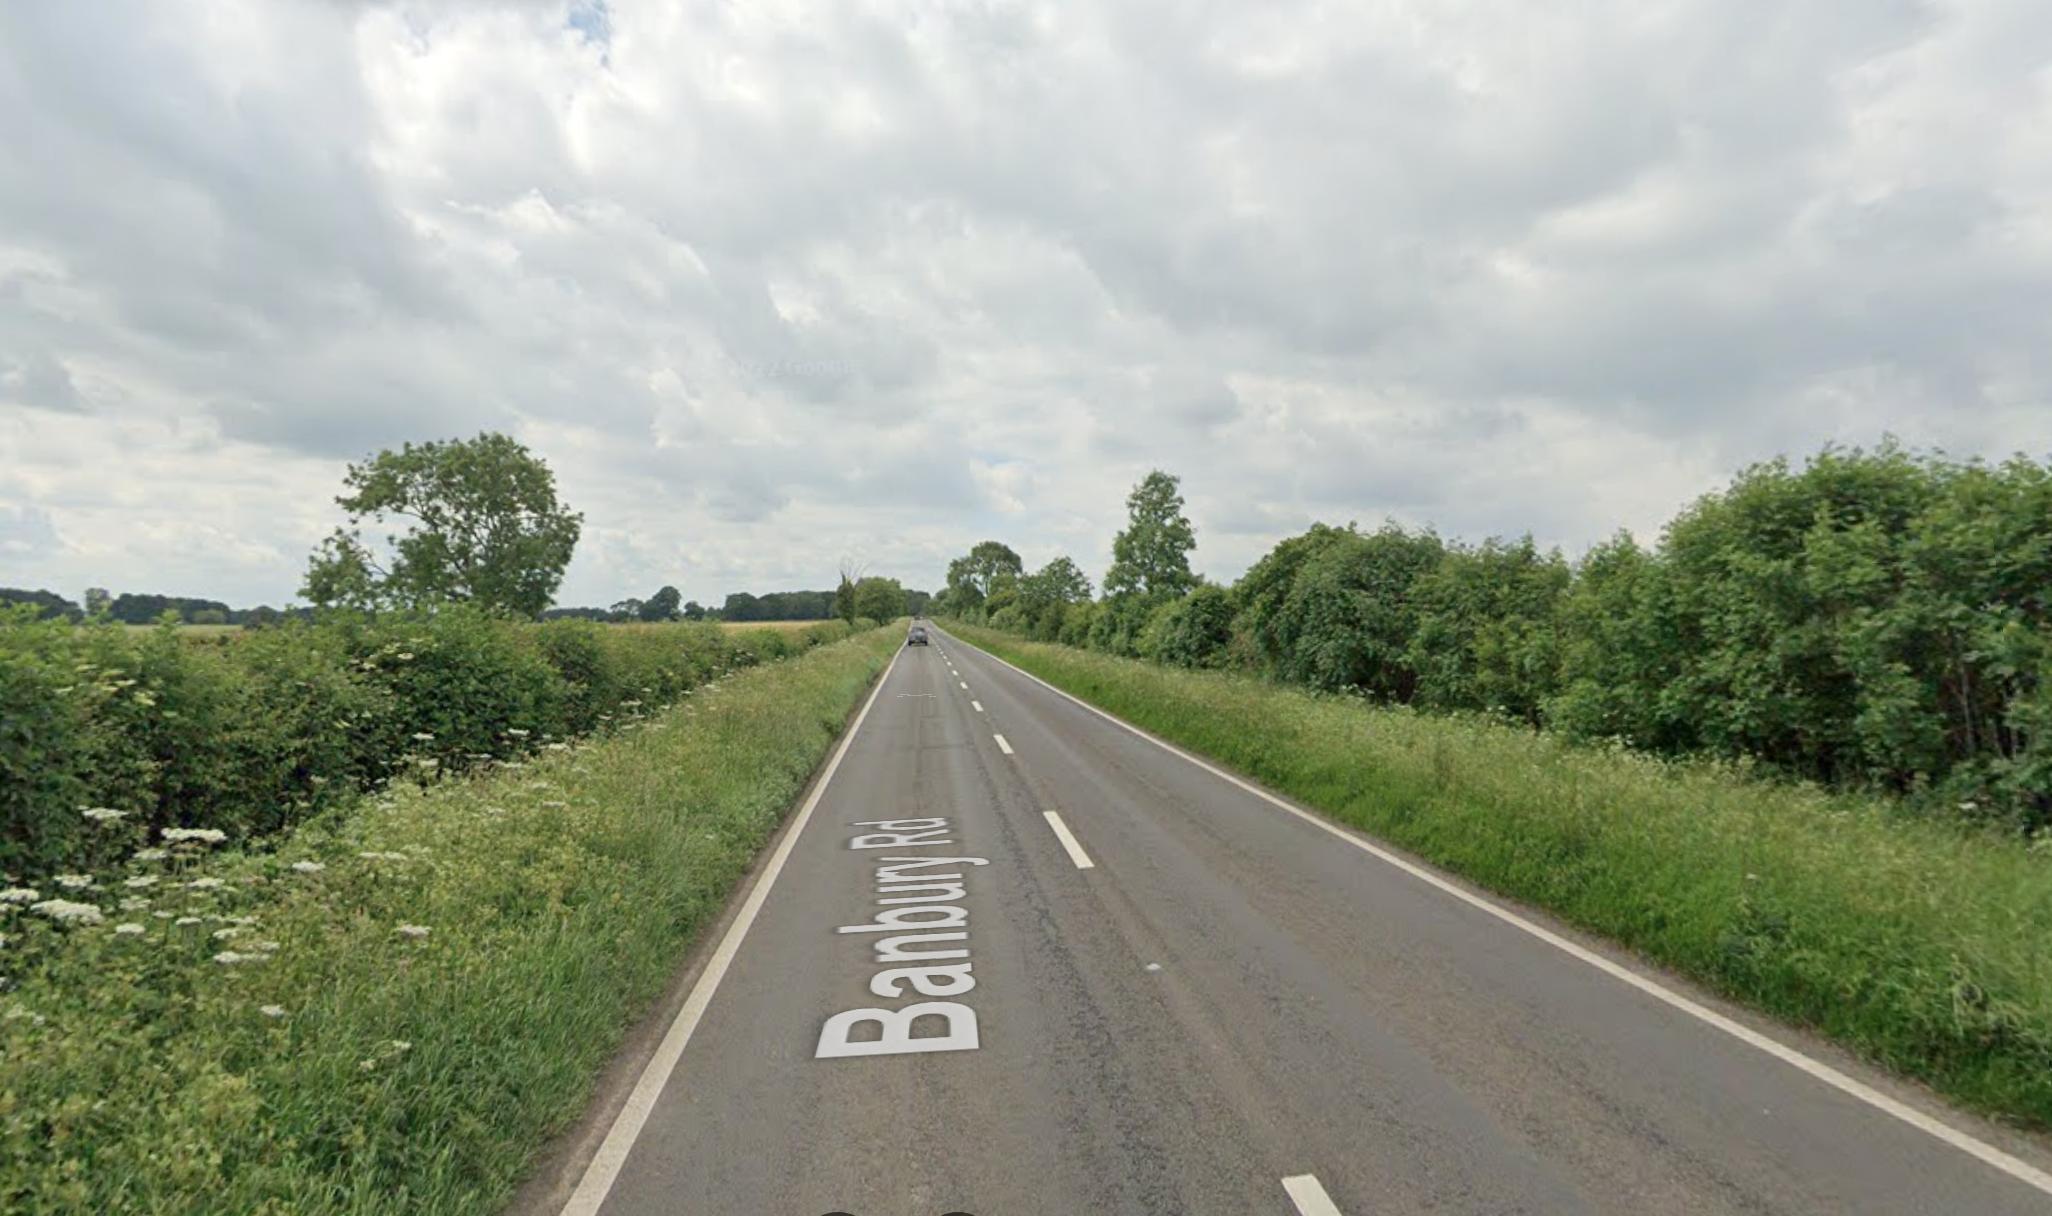
\includegraphics[height=.7\textwidth, width=\textwidth]{images/UnlabelledDemo1.png}
        \\ \includegraphics[height=.7\textwidth, width=\textwidth]{images/LabelledDemo1.png}
    \end{minipage}
    \begin{minipage}{.3\textwidth}
        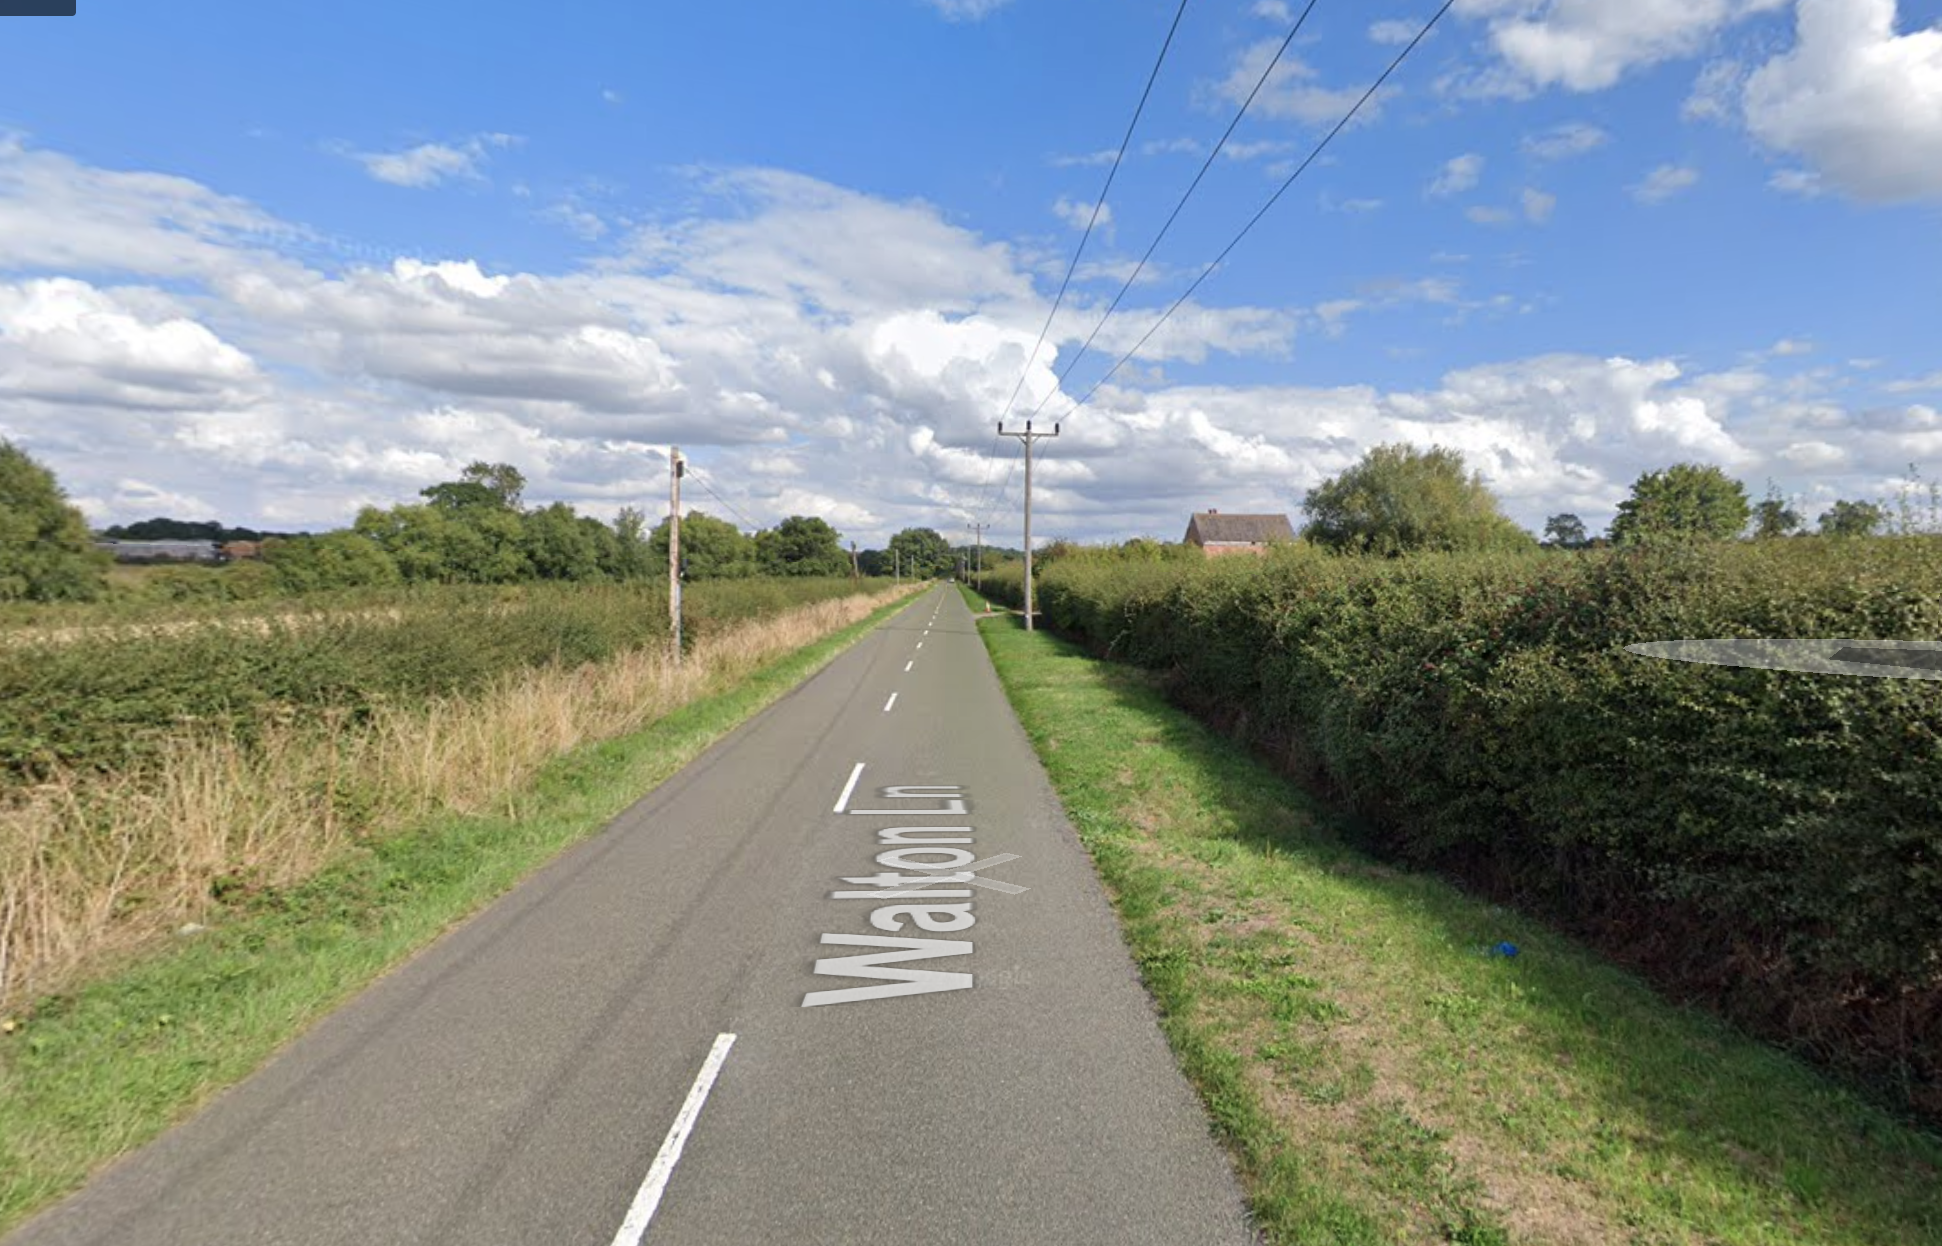
\includegraphics[height=.7\textwidth, width=\textwidth]{images/UnlabelledDemo2.png}
        \\ 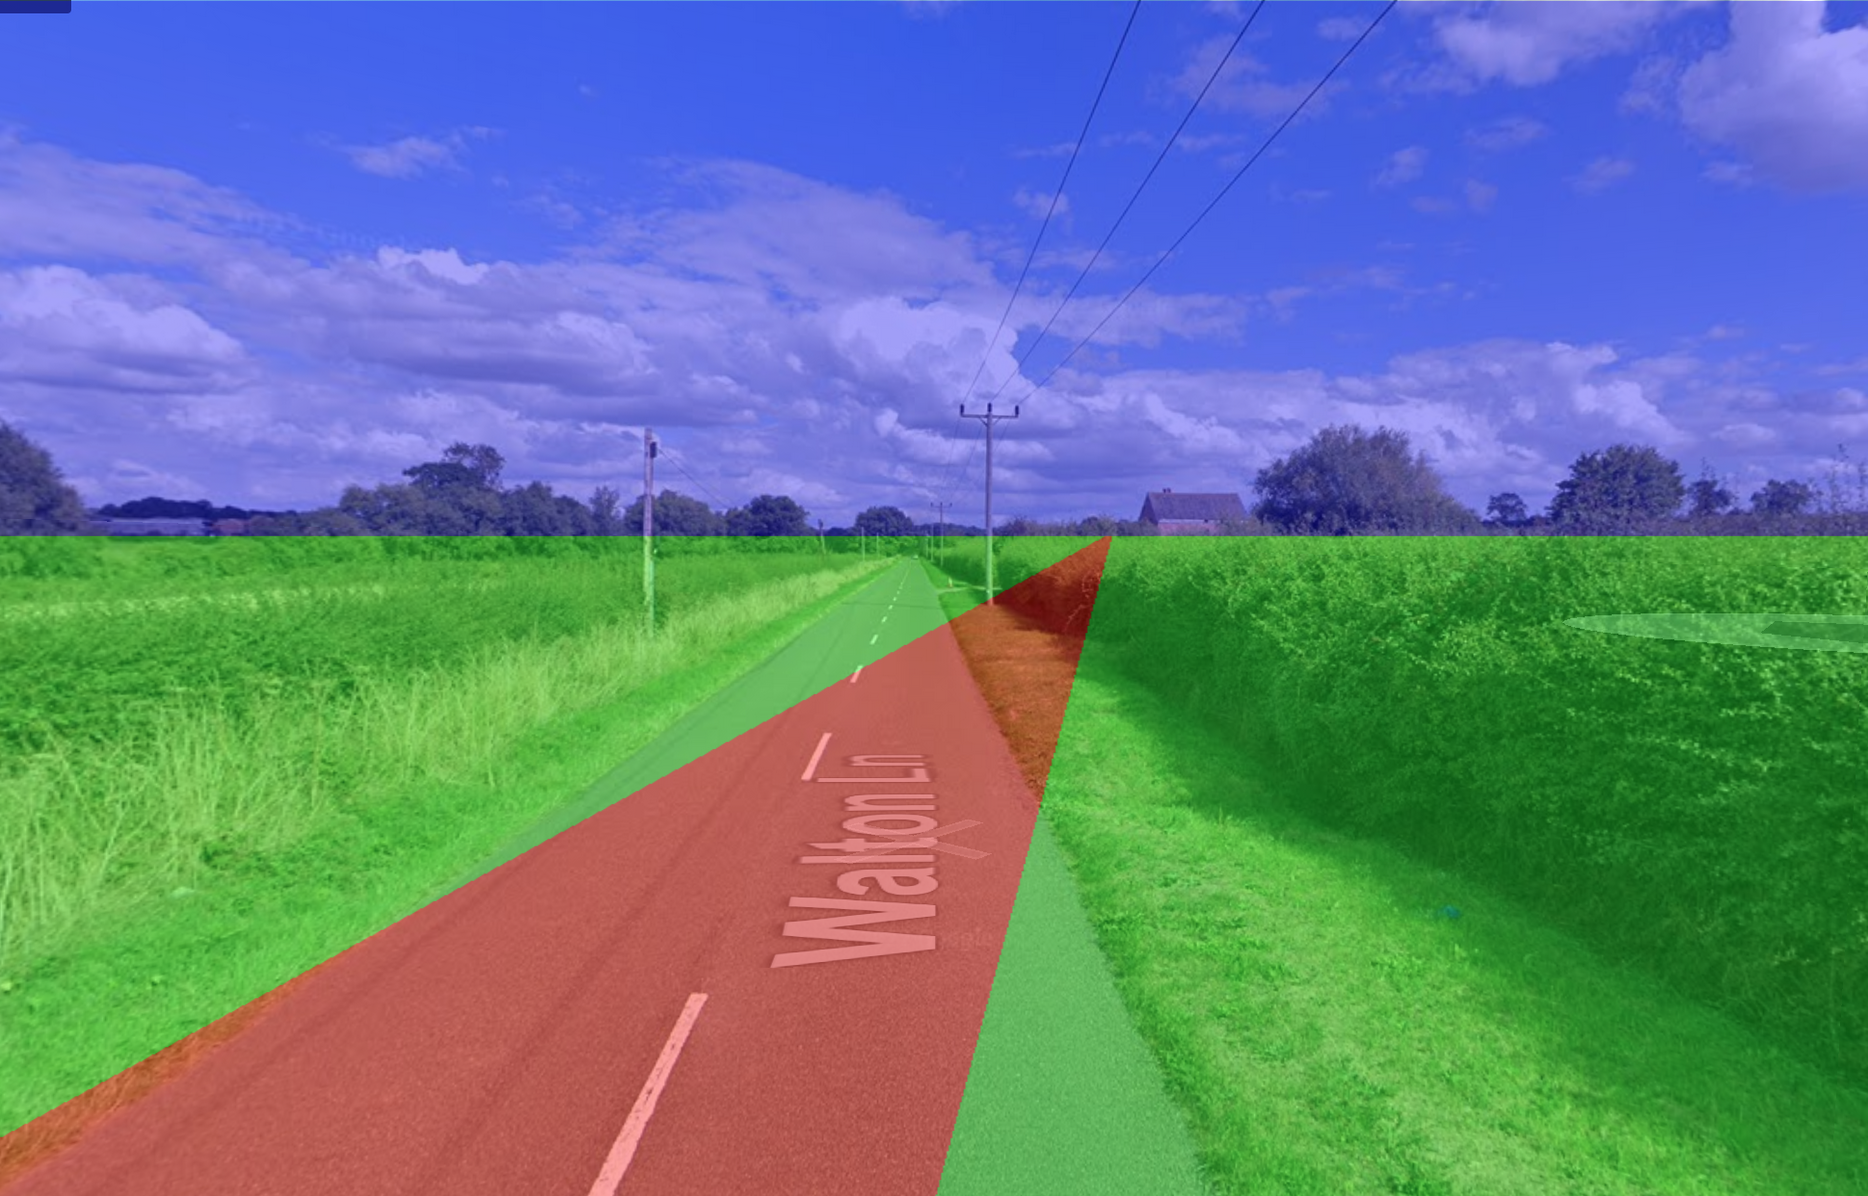
\includegraphics[height=.7\textwidth, width=\textwidth]{images/LabelledDemo2.png}    
    \end{minipage}
    \begin{minipage}{.3\textwidth}
        \includegraphics[height=.7\textwidth, width=\textwidth]{images/UnlabelledDemo3.png}
        \\ \includegraphics[height=.7\textwidth, width=\textwidth]{images/LabelledDemo3.png}    
    \end{minipage}
    \caption{Labelled Images}
    \label{fig:labelresults}
\end{figure*}

\section{Produced Work}
\begin{figure*}[h]
    \centering
    \includegraphics[width=.9\linewidth]{images/FFI Diagram.drawio.pdf}
    \caption{The structure of the road marking labeller}
    \label{fig:ffidiagram}
\end{figure*}

The code for all the artifacts mentioned can be found within the \href{https://github.com/Functional-Labelling-Lab}{Functional Labelling Lab} GitHub organisation.

\subsection*{\textbf{FusedProbFX}}
One of the primary artifacts of the project is the re-implementation of the existing ProbFX library using the algebraic effects framework fused-effects. In discussing the architecture of our implementation here, we assume some knowledge on the topics of algebraic effects and the implementation of the fused-effects library. Additional information and explanations can be found in appendices \ref{app:AlgebraicEffectsAppendix} and \ref{app:FusedEffectsAppendix} respectively.

\subsection*{Overview of ProbFX}
The ProbFX library allows for a great degree of flexibility in probabilistic programming. It allows users to write composable, modular probabilistic models that can both sample and observe the primitive distributions they are constructed from. The dynamic nature of the DSL is possible thanks to its foundations being implemented using algebraic effects. ProbFX uses 3 main effects to implement its provided features:

\begin{enumerate}
    \item \textbf{ObsReader} is responsible for implementing observation of probabilistic variables. It does this by taking their values from an environment, which contains lists of values for each random variable that the model should observe consecutively along its execution. Sampling from primitive distributions is achieved by not supplying any observed values for a specific random variable in the environment.
    \item \textbf{SampObs} is responsible for the implementation of sample and observe actions for the different algorithms that ProbFX can run. For example tracing the runtime addresses of calls to different random variables, or simply providing a means of sampling from a given model.
    \item \textbf{Dist} is responsible for the top-levels dispatch of calls to SampObs by different primitive distribution functions. It also calculates data that SampObs implementations later use. Some examples are
    the runtime addresses of the random variable samplings, whether a particular random variable should be called, or whether a particular random variable should be sampled from a primitive distribution or observed from the environment.
\end{enumerate}

ProbFX was originally written for a research project, as a proof-of-concept of the application of algebraic effects to probabilistic programming. It uses a custom Freer monad-based implementation, which, while simple and elegant, suffers in performance and interoperability with other systems.

\subsection*{Re-implementing ProbFX with fused-effects}

Our work on the library was focused on making it production-ready by increasing its interoperability with other Haskell libraries and providing a more user-friendly interface. This was achieved by changing ProbFX's effect implementation from a custom Freer monad-based implementation to a fused-effects based one. We also attempted to switch the ObsReader effect to a dependently typed union of effects, which would have worked similarly to how a type union \cite{higherrinductivetypes} can hold information about all the different types it is defined over. This however proved impossible currently due to incompatibilities in GHC versions and time constraints on the project.

\subsection*{Other improvements over ProbFX}
Aside from the porting of the library's effect system to fused-effects, there were several less complex changes made to the library with the goal of production-readiness:
\begin{itemize}
    \item We added transition models for resampling the random variables in the library's implementation of the Metropolis Hastings algorithm.    
    \item We switched the Environment's implementation to an external library for product types \cite{higherrinductivetypes}.
    \item We made some smaller ergonomic improvements such as Metropolis Hastings iterations being indexed on the number of successful variable resamplings, rather than resampling trials. We also simplified and reorganized some redundant modules originally present in the library. 
\end{itemize}

\subsection*{\textbf{Road Marking Detection}}

The other main section of our project was the application of fused-probfx to a non-trivial issue. We implemented an image labelling pipeline which makes extensive use of fused-probfx and Metropolis Hastings, a Markov Chain Monte Carlo (MCMC) method. Additional information on this probabilistic inference technique can be found in Appendix \ref{app:MetropolisHastingsAppendix}.

\subsection*{Labelling Pipeline}
The pipeline for our image labeller is relatively simple, as can be seen in Figure \ref{fig:pipeline}. We first load our target image from the local file system. We then apply a pre-processing stage to the image in order to improve the ease with which we can calculate the estimation error. After the pre-processing is complete, we begin the iterative process of using fused-probfx to sample a road scene from the constructed model. These road scenes are then rendered and compared to our pre-processed target image, producing an error value describing how well the rendered scene corresponds to the real-world image. This error can then be used to update our model with Metropolis Hastings. After we have finished an initial burn-in period, we keep updating the model until it has converged to a suitable minimum error. The stages of this pipeline are explained in greater detail below.

\begin{figure}[h]
    \centering
    \includegraphics[width=\linewidth]{images/pipeline.drawio.pdf}
    \caption{Image Labelling Pipeline}
    \label{fig:pipeline}
\end{figure}

\subsection*{Target Image Pre-processing}
Comparing real images to synthetic images is a difficult task, and the surrounding literature suggests that the problem is very domain specific. As Metropolis Hastings requires an error to minimize, we employed the following techniques to pre-process the real images before comparing them to the synthetic images:
\subsection*{K-Means-Clustering}
K-means-clustering is a compression algorithm, where k pixel values are randomly selected as centroids in the RGB space, and the image pixels are updated to be the closest centroid. Centroids are then updated to be the average value of their assigned image pixel groups. The process is repeated until convergence. The resulting image only contains k distinct colours, which decreases pixel-to-pixel noise.
\subsection*{Direct Colour Assignment}
Direct colour assignment is another compression algorithm, specifically devised for this project. The algorithm employs the domain-specific information that the surroundings of most roads are more green, roads are typically more brown/black, and the sky is typically more blue. We then polarize the pixels of the image to be one of three target colours, which decreases noise. This is in effect a form of domain-specific semantic image segmentation. This was the most successful compression algorithm. 

\subsection*{Hough Transform}
In order to reduce project risk, we also experimented with using line comparison on images to generate additional error metrics. To do this we used Hough Line Extraction from OpenCV to detect the dominant lines in the target image, and then compared the geometry of these lines to the geometry from our rendered scene. While this ultimately did not give better results, it provides an additional possible error metric to aid in convergence. A full system diagram, demonstrating all approaches trialed, is show in Figure \ref{fig:ffidiagram}.

\begin{figure}[h]
    \centering
    \includegraphics[width=\linewidth]{images/preprocessing.png}
    \caption{Different image pre-processing methods. Top-Left: Input image, Top-Right Hough Transform, Bottom-Left: K-means clustering with k = 10, Bottom-Right: Direct colour assignment}
    \label{fig:kmeans}
\end{figure}

\subsection*{Scene Rendering}
In order to determine the accuracy of our predicted road scene ("the error") we compare the target image with a render generated from the model's predicted parameters. To do this we use our scene renderer, written in C/C++ and OpenGL.

The renderer takes as input the parameters used to describe the positioning of the camera observing the road, producing a simple, block-colour render of the road. Due to the iterative nature of Metropolis Hastings, this rendering must occur many thousands of times, and so high performance code is imperative. It is for this reason that we have implemented our renderer with OpenGL. This is despite the associated development costs of working with a lower-level framework. We go into more detail on why we choose OpenGL in Appendix \ref{app:unityopengl}.

\subsection*{Error}

After rendering, our scene is separated into different channels for different sections of the scene; for example, a channel each for the road, sky and surroundings, as shown in Figure \ref{fig:imagerend}. We use a shader inside OpenGL to achieve this, allowing for performant comparison of the different elements of the scene to the target image independently, which increases the accuracy of the calculated error. 

\begin{figure}[h]
    \centering
    \includegraphics[width=\linewidth]{images/labelled render.png}
    \caption{Image Rendering with OpenGL}
    \label{fig:imagerend}
\end{figure}

\section{Evaluation}

\subsection*{Road Marking Detection}
Overall, we feel that we have successfully demonstrated the viability of our stack in a real-world use case. The requirement from Ghost Autonomy was for proof-of-concept road labelling, and as such we designed our evaluation methodology around this. We met frequently with Ben Lippmeier, to ensure the software aligned with his requirements, and have implemented into the project a number of evaluation metrics.

Our primary evaluation method was visual inspection of mask outputs of the model, to allow for qualitative, at-a-glance validation of the accuracy of the model by a user.

To aid iteration, we also provide a synthetic benchmarking suite, where synthetic renders are generated, road markings are inferred from them, and the accuracy of this inference is scored. This process allows for a quantitative measure of performance, aiding in the client's use case of experimenting and developing detection models. This process is demonstrated in Figure \ref{fig:synthetic}.

The package overall is easy to use; it processes entire directories at once as well as individual images, and outputs a single, summary CSV file. It affords great flexibility, as thanks to fused-probfx the model can be easily modified, and the entire stack is generic over the type of error function, all aiding experimentation and ease of development.

We hoped as an initial goal to target more complex road scenes, including curved and multi-lane roads, however this did not end up being feasible in the available time.

\begin{figure}[h]
    \begin{center}
    \begin{minipage}{.49\linewidth}
        \includegraphics[width=\textwidth]{images/SyntheticInput.png}    
    \end{minipage}\hfill%
    \begin{minipage}{.49\linewidth}
        \includegraphics[width=\textwidth]{images/SyntheticOutput.png}
    \end{minipage}
    \end{center}
    \vspace{2mm}
    Benchmark $n=10$ (Avg. Euclidean scene difference: $1.0135$, Std. dev: $0.56137$)
    \caption{Synthetic benchmarking: Synthetic target (left) and Inferred result (right)}
    \label{fig:synthetic}
\end{figure}

\subsection*{fused-probfx}

One of the primary problems with the original ProbFX was that its Freer monad-based implementation of algebraic effects was custom and incompatible with other effectful libraries. Changing that backend to fused-effects made the project compatible with other libraries using it. As a result, one function could have side effects as specified by our library, as well as an arbitrary 3rd party library's effects. Since there are already multiple libraries \cite{FusedEffects} [Contributing Packages] using fused-effects as a backend, this adds a significant amount of inter-operability and outreach to the library.

Re-implementing ProbFX with fused-effects has also moved some of the maintenance burden and performance tuning work out of the library to fused-effects. This leaves less technological baggage in fused-probfx and encourages further feature expansion of the library by other developers.

The other major reason for re-writing ProbFX using fused-effects was performance. While fused-effects by itself is much faster than the Freer monad method ProbFX uses, as show in Figure \ref{fig:effectsbenchmarks}, we have not had sufficient time to make use of these performance optimisation opportunities. This leaves our re-write slower than the original ProbFX when compared using a standard benchmark to a number of other PPLs; We are however confident that the only performance relevant differences between ProbFX and fused-probfx are the effects system, and that fused-probfx will eventually enjoy a significant speed advantage due to potential provided by fused-effects.

\begin{figure}[h]
    \centering
    \includegraphics[width=\linewidth]{images/effect_library_comparison.png}
    \caption{Time per iteration for 4 of the effect systems compared by \cite{effectsbenchmarks}.}
    \label{fig:effectsbenchmarks}
\end{figure}

The smaller improvements to the Metropolis Hastings algorithm significantly improved the performance and ergonomics of using it in the road marking detection section of the project, by reducing the burn-in period needed and making it easier to fine-tune the behavior of the algorithm.

Finally, converting the Environment to use a generalized product type implementation allowed for a more uniform implementation of other extensions to the library, such as transition models for Metropolis Hastings, easier mapping between the two Product types, and greater expressiveness of type-level constraints for the lists of random variables over which the different product types are defined.

\section{Build}
Due to the complex multi-language nature of the project, fused-probfx and the road marking labeller are built separately and then combined. fused-probfx is built with Cabal and the road marking labeller is built with CMake. A diagram illustrating this build process is included as Appendix \ref{app:build}

\bibliographystyle{vancouver}
\bibliography{refs}

\newpage
\appendices

\section{Algebraic Effects}
\label{app:AlgebraicEffectsAppendix}
Effect types attempt to give exact semantics and type safety to the side effects of functions. A given effect does this by defining a set of actions that can be executed by an effectful computation with said effect in its type signature. For example, a function which has a side effect on the file system might have a \texttt{FileSystem} effect in its type signature, which allows the running of two functions, \texttt{ReadFile} and \texttt{WriteFile}. \texttt{ReadFile} and \texttt{WriteFile} are effectful computations that can only be executed within other effectful computations that have the \texttt{FileSystem} effect. A handler can then be applied on the effectful computation to produce a computation without the associated effect, and with the effect's syntax replaced with a call to the handler. 

Algebraic effects may be used similarly to monads, for example the IO monad, which allows for reading and writing from the file system. They however differ from monads in two important ways:
\begin{enumerate}
    \item Effects separate a computation's semantics from its syntax. As a result, when constructing an effectful computation, it is not required to specify what handler will be used for any given effect. The handlers are the concrete implementations of each of the effect's actions.
    \item A computation can have many associated effects, in no particular order. This contrasts with monads, where monadic functions can only have one set of side effects. Monad transformers attempt to resolve this by allowing several monads to be composed; this however enforces a rigid ordering of monads which harms the ergonomics of using them.
\end{enumerate}

A helpful way to think about an effectful computation is as a computation which uses multiple monads and is generic over their implementation and order.

\section{fused-effects}
\label{app:FusedEffectsAppendix}
There are many ways to express effect types in Haskell. The most common way in existing literature, although not in production code, is the Freer monad. The Freer monad works by representing effectful computation as a tree, where every leaf is a pure value, and every branch is an effectful action and the continuation of the computation. To run such a tree, all branches in a tree are recursively replaced, one-by-one, with a call to a handler for their corresponding effect, which is also given a continuation. Once all effects are handled, only a leaf remains in the tree, representing the result of the computation.

The problem with this approach is the runtime nature of the Freer monad. With each new computation constructed, the method has to recurse over the entire computation tree to handle that effect. This transformation is expensive; slower than an equivalent monad transformer-based computation. To solve this, fused-effects \cite{FusedEffects} uses a method described in \cite{fusionforfree} which changes how calls to effectful computations are handled: instead of implementing semantic polymorphism of effects at runtime, the method achieves the desired effects with polymorphism over a monad which the computation is wrapped in, and specialization of said monad at the execution site of the computation at compile time. This is done by specifying a stack of monad transformers called "Effect Carriers" that implement the effects required by the polymorphic computations.

\section{Metropolis Hastings}
\label{app:MetropolisHastingsAppendix}
The Metropolis Hastings algorithm is a probabilistic technique implemented in fused-probfx and used heavily in the Road Marking detection section. Metropolis Hastings is a part of a family of algorithms known as Markov Chain Monte Carlo algorithms. They allow for the sampling of a specific distribution while only knowing its un-normalised density function, i.e. an $f(x)$ such that $f(x)/p(x)$ is constant, where $p(x)$ is the actual density function of the distribution. This property is particularly useful when sampling custom, composite distributions. It's not always possible to know the exact density function of a distribution, but knowing a function proportional to the density function is much easier. Metropolis Hastings works by re-sampling a given random variable from a probabilistic model using some transition model and then randomly deciding whether to keep a given re-sampled value \cite{methastings}. The probability of keeping a given re-sampled value is calculated based on the conditional probabilities of the re-sampled values occurring within the model. 

\section{Why OpenGL}
\label{app:unityopengl}
Coming into the project with little to no group experience in OpenGL it definitely could be argued that it may have been wiser to user a higher-level ecosystem such as Unity. This would have however had its own issues; it would have added significantly more bloat and complexity to a project that already had a complex build system. It also most likely would have been significantly slower than OpenGL.

As OpenGL is so widely supported by hardware manufacturers it is effectively guaranteed to be available on any modern-day machine. We did however encounter challenges with OpenGL compatibility over different operating systems, with WSL not yet supporting OpenGL versions above 3.3 other than with integrated CPU graphics. OpenGL is also highly optimised and provides an easy interface to processing on the GPU, which is critical for our compute-heavy rendering.


\begin{figure*}[h]
\section{Build Diagram}
    \centering
    \includegraphics[width=\linewidth]{images/Build System.png}
    \label{app:build}
\end{figure*}

\end{document}
